\documentclass[aps,twocolumn,prl,showpacs,showkeys,preprintnumbers,superscriptaddress,nobibnotes,floatfix,longbibliography,notitlepage,nofootinbib]{revtex4-2}

\usepackage{graphicx}
\usepackage{epstopdf}
\usepackage{amsmath}
\usepackage{amsfonts}
\usepackage{amssymb}
\usepackage{appendix}
\usepackage{enumerate}
\usepackage{natbib}
\usepackage{comment}
\usepackage{bbold}
\usepackage[shortlabels]{enumitem}
\usepackage{color}
\usepackage{slashed}
\usepackage{subfigure}
\usepackage{setspace}
\usepackage{footnote}
\usepackage{lipsum}
\usepackage{multirow}
%\usepackage{longtable}
\usepackage[colorlinks = true,
            linkcolor = blue,
            urlcolor  = blue,
            citecolor = blue,
            anchorcolor = blue]{hyperref}
\usepackage[capitalize]{cleveref}
\usepackage{braket}
% \usepackage[compat=1.1.0]{tikz-feynman}
\usepackage{multirow}
\usepackage{physics}
% \usepackage{feynmp-auto}
\usepackage[normalem]{ulem}
\usepackage{url}
\usepackage{units}
\usepackage[normalem]{ulem}
\newcommand{\yy}[1]{\color{red}[YY:#1]\color{black}}



\usepackage{graphicx}% Include figure files
\usepackage{dcolumn}% Align table columns on decimal point
\usepackage{bm}% bold math
%\usepackage{hyperref}% add hypertext capabilities
%\usepackage[mathlines]{lineno}% Enable numbering of text and display math
%\linenumbers\relax % Commence numbering lines

%\usepackage[showframe,%Uncomment any one of the following lines to test 
%%scale=0.7, marginratio={1:1, 2:3}, ignoreall,% default settings
%%text={7in,10in},centering,
%%margin=1.5in,
%%total={6.5in,8.75in}, top=1.2in, left=0.9in, includefoot,
%%height=10in,a5paper,hmargin={3cm,0.8in},
%]{geometry}
\usepackage{lipsum}
\usepackage{lettrine}
\begin{document}

\preprint{USTC-ICTS/PCFT-24-07, APS/123-QED}
\bibliographystyle{apsrev4-1}
\title{
% New Physics in Supernovae at Neutrino Telescopes
% Time Prints of New Physics from Supernovae at Neutrino Telescopes
% Supernova Detection with Neutrino Telescopes as a Portal to New Physics
Supernovae Time Profiles as a Probe of New Physics at Neutrino Telescopes
}

\author{Jeff Lazar}
\email{jlazar@icecube.wisc.edu}
\affiliation{Department of Physics \& Laboratory for Particle Physics and Cosmology, Harvard University, Cambridge, MA 02138, USA}
\affiliation{Department of Physics \& Wisconsin IceCube Particle Astrophysics Center, University of Wisconsin-Madison, Madison, WI 53706, USA}
\author{Ying-Ying Li}
\email{yingyingli@ustc.edu.cn}
\affiliation{Peng Huanwu Center for Fundamental Theory, Hefei, Anhui 230026, China}
\affiliation{Interdisciplinary Center for Theoretical Study, University of Science and Technology of China, Hefei, Anhui 230026, China}
\author{Carlos A. Arg\"{u}elles}
\email{carguelles@g.harvard.edu}
\affiliation{Department of Physics \& Laboratory for Particle Physics and Cosmology, Harvard University, Cambridge, MA 02138, USA}
\author{Vedran Brdar}
\email{vedran.brdar@okstate.edu}
\affiliation{Department of Physics, Oklahoma State University, Stillwater, OK, 74078, USA}

%\date{\today}

\begin{abstract}
Neutrino telescopes, including IceCube, can detect galactic supernova events by observing the collective rise in photomultiplier count rates with a sub-second time resolution. Leveraging precise timing, we demonstrate for the first time the capability of neutrino telescopes to explore new weakly coupled states emitted from supernovae and subsequently decaying to neutrinos. Our approach utilizes publicly available packages, \texttt{ASTERIA} and \texttt{SNEWPY}, for simulating detector responses and implementing neutrino fluxes originated from Standard Model and new physics. We present results for two new physics models
employing a specific supernova model and introduce the tool developed for testing a diverse range of new physics models.
\end{abstract}

%\keywords{Suggested keywords}%Use showkeys class option if keyword
                              %display desired
\maketitle
\textbf{\textit{Introduction}}---
The Standard Model (SM) is a remarkable but incomplete theory. Puzzles such as the non-vanishing tiny neutrino mass, the origin of observed matter-antimatter asymmetry, and the nature of dark matter, among others, all seek explanations beyond the Standard Model (BSM). However, there are no affirmative clues for the energy scale the yet undiscovered particles should appear. Numerous BSM searches across the scales have been performed, from collider searches at high energies \cite{Nath:2010zj} to studies of cosmic microwave background at temperatures near absolute zero \cite{Baumann:2015rya}. Galactic SN explosion, where majority of emitted energy is released in the form of neutrinos, offers unique opportunities in testing BSM physics via interactions with active neutrinos. So far we have observed SN 1987A in neutrinos. The duration of such a signal \cite{Kamiokande-II:1987idp,Bionta:1987qt,Baksan} as well as the inferred total emitted energy \cite{Loredo:2001rx,Pagliaroli:2008ur,Huedepohl2010} allow us already to set a tentative constraint on the energies that could be taken away from any light BSM particle copiously produced in the interior of a star. Indeed, many different BSM scenarios models have been constrained in this way, see \emph{e.g.} \cite{Raffelt:2011nc,Arguelles:2016uwb,Suliga:2020vpz,Lucente:2021hbp,Caputo:2022rca,Caputo:2021rux,PhysRevD.100.083002,DeRocco:2019njg,Kazanas:2014mca,Magill:2018jla}.

If, additionally, new physics particles, emitted from the SN core, can decay to neutrinos, even stronger limits can be set. In particular, for the standard case, neutrinos interact frequently in the core and eventually leave the star with $\mathcal{O}(10)$ MeV energy. New states after being produced can stream out without further interactions. Consequently, they typically exit with higher energies, subsequently decaying into neutrinos with an energy on the order of $\mathcal{O}(100)$ MeV. Limits can be set from the fact that such high energy neutrinos were not recorded from SN 1987A \cite{Kamiokande-II:1987idp,Bionta:1987qt,Baksan, Fiorillo:2022cdq, Brdar:2023tmi}. Once produced from SN, the new state can be non-relativistic and travels slowly, causing time delays to the arrival time of its daughter particle which was also recently employed \cite{Brdar:2023tmi} for a time window around one day. However, as being decoupled immediately, it is possible that new states can exit the supernova at an earlier time instead—an effect that has not been previously considered. These two effects in combination would cause advanced or delayed neutrino signals to the standard case.

On the other hand, neutrino telescopes such as IceCube have not only pioneered in detecting neutrinos at ultra-high energies \cite{IceCube:2014stg,IceCube:2018cha} and from specific extragalactic sources \cite{IceCube:2023ame,IceCube:2022der},but also in testing temporal correlation of MeV neutrino events with fast radio bursts \cite{IceCube:2019acm} by detecting a collective rise in all photomultiplier rates within a time window as short as 0.01 second on the top of the background noise. In this work, we demonstrate that such precise time resolutions will play a crucial role in tracking the delayed neutrino signals, and interestingly reveil new features of advanced neutrino signals coming from the immediate-decoupling of its mother particles. This novel timing patterns generically exist in models with new weakly interacting particles, such as the aforementioned Majoron models \cite{Fiorillo:2022cdq}, sterile neutrino via the dipole portal \cite{Magill:2018jla,Brdar:2020quo,Brdar:2023tmi} or mixing portals \cite{Arg_elles_2019, Suliga_2020}. Once produced inside the SN, these particles stream out at an earlier time than the standard neutrino signal. Meanwhile, for non-negligible mass, they would travel slower than active neutrino before decaying or converting back to active neutrinos. Via the timing measurement, we will show that neutrino telescope can provide unprecedented constraints on the parameter space in BSM.\\ 
\textbf{\textit{The Models}}---
Let us start by discussing aforementioned new physics models in more detail.
The first scenario under consideration is active-to-sterile neutrino transition magnetic moment described by \cite{Magill:2018jla,Brdar:2020quo,Brdar:2023tmi}
\begin{align}
    \mathcal{L} \supset \sum_\alpha d_\alpha \bar{N}\sigma_{\mu\nu} \nu^{\alpha} F^{\mu\nu}-\frac{M_N}{2} \bar{N}^c N + \text{h.c.}\,,
    \label{eq:Lag}
\end{align}
where $\nu^{\alpha}$ and $N$ represent active and sterile neutrinos, respectively. Further, $F^{\mu\nu}$ is the field strength tensor of the electromagnetic field and $d_\alpha$ is the dimensionful coefficient of this dimension-5 term and $M_N$ is sterile neutrino mass. We will abbreviate $d_\alpha \equiv d$ given that we assume flavor universal interaction. The dominant production channels for $N$ inside the SN are $\nu e^- \to \nu e^-$ at lower energies and $\nu \gamma \to N$ for larger active neutrino energies. Both processes occur due to the interaction term in \cref{eq:Lag}; after $N$ are produced, they decay to active neutrinos and photons which is again realized through the same term in the Lagrangian, with the decay width for $N\to\nu\gamma$ given by $\Gamma_N = 6d^2 M_N^3/4 \pi$ \cite{Plestid:2020vqf}. 

The second model that will be analyzed in this work is the Majoron model from \cite{Fiorillo:2022cdq}. The relevant part of the Lagrangian reads
\begin{align}
\mathcal{L} \supset -\frac{g_{\alpha\beta}}{2} \nu_\alpha \nu_\beta \phi - M_\phi \phi\phi^* + \text{h.c.}\,,
\end{align}
where $M_\phi$ is the Majoron mass and $g$ parametrizes interaction strength between $\phi$ and neutrinos. As in the previous model, we assume flavor universal interaction, hence we abbreviate $g_{\alpha\beta}\equiv g$. Majorons are produced from neutrino coalescence in the star and then subsequently decay to a pair of neutrinos with the total decay width to all flavor of neutrinos given by $\Gamma_\phi = 3g^2 m_\phi/16 \pi$, and as a result, BSM neutrino flux is produced. 


%The differential number of sterile neutrinos $\mathcal{N}_s$ produced per unit time $t$ at position $r$ is \cite{Arguelles:2016uwb}
%\begin{align}
%\frac{1}{4\pi r^2}\frac{\partial^2}{\partial r\partial t}\left(\frac{d\mathcal{N}_s}{dE_N}\right)= \sigma n_\nu \frac{d n}{dE}\,.
%\label{eq:simplified}
%\end{align}
%where $\sigma n_\nu$ is the interaction rate for the production process with $n_\nu$ being the number densities of the neutrino. $n$ is the number density of electron (neutrino) for sterile neutrion $N$ (Majoron $\phi$) production. 
Using data simulated by the Garching group for an $8.8 M_\odot$ progenitor star \cite{Huedepohl2010}, we obtained the fluxes of sterile neutrino $N$ and Majoron $\phi$, and produced the cooling limit as depicted in Fig. \cref{fig:exclusion}. The results are in agreement with those obtained in literature \cite{Fiorillo:2022cdq, Brdar:2023tmi}.
%, with the  ``cooling'' bound depicted in \cref{fig:exclusion} (gray region).
%Requiring the total energy carried away by $N$ to be less than $10\%$ of the total available neutrino energy leads to the  ``cooling'' bound depicted in \cref{fig:exclusion} (gray region). Our estimate is in agreement with the one obtained in \cite{Fiorillo:2022cdq, Brdar:2023tmi}. 
As we are interested in cases where the coupling strength is below the cooling limit, these new states once produced in the SN core will stream out without further interacting with SN plasma before decaying.
 For a given emission angle $\alpha$ of daughter neutrino relative to the direction of mother particle, and the angle $\theta$ at which the daughter neutrino arrives at the Earth, the time delay $\Delta t$, the arrival time of the daughter $\gamma$/$\nu$ relative to that of the neutrinos produced in the explosion via SM processes, is \cite{Jaeckel:2017tud}
\begin{align}
    \Delta t = L_1/\beta + D_{\rm SN} \cos\theta-L_1 \cos\alpha -D_{\rm SN}\,,
    \label{eq:deltat}
\end{align}
with $D_{\rm SN}$ the distance between the SN and the Earth, and $L_1$ the distance mother particles propagated before decaying.
The flux of daughter $\nu$ is obtained by considering decays that only occur at $R^{\gamma/\nu}_{\rm SN}\leq L_1 \leq L^{\rm max}_1$. As the smallest decay distance beyond which the daughter neutrino can escape the explosion unperturbed, we take $R^{\nu}_{\rm SN} = \unit[30]{km}$.
$L^{\rm max}_1$ corresponds to the distance $L_1$ with the largest time delay $\delta t = \unit[100]{s}$ while larger values of $\delta t$ do not affect the limits obtained. For the time delay bounded by $\delta t = \unit[100]{s}$, $\theta < 5^\circ$ \cite{Brdar:2023tmi}. We show the fluxes of daughter neutrino in comparison to the standard neutrino flux in Fig. \cref{fig:fluxes}.

\begin{figure}[t!]
    \centering
    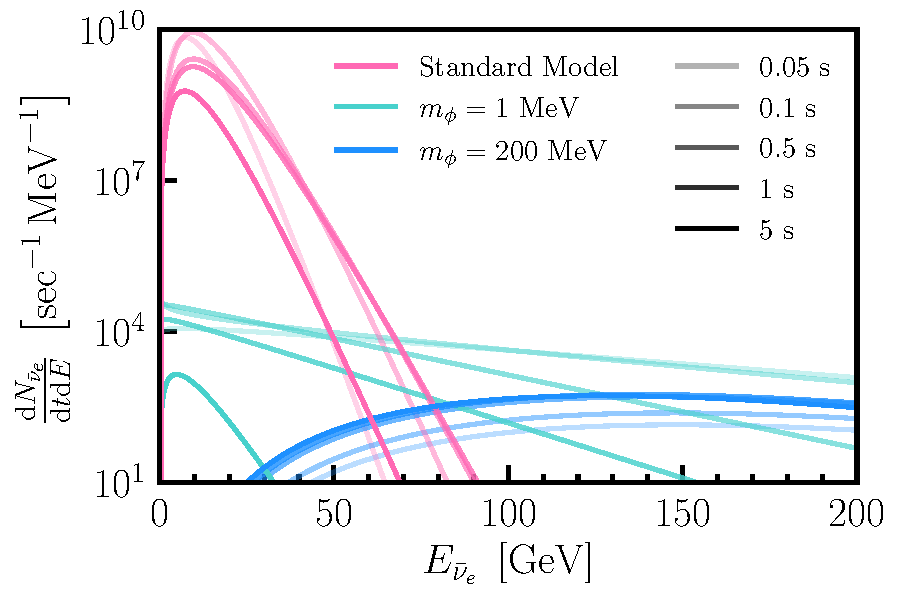
\includegraphics[width=0.47\textwidth]{figures/majoran_fluxes.pdf}
    \caption{\textbf{\textit{Neutrino flux from Standard Model production and two majoran hypotheses.}}
    Jeff needs to write here.
    }
    \label{fig:fluxes}
\end{figure}
\textbf{\textit{Detector Response and Statistical Treatment}}---
% The first step in our processing chain is to attain $\nu_{e}$, $\bar{\nu}_{e}$, and $\nu_{X}$ fluxes at the detector.
% These should take the form of the flux---in units of $\mathrm{MeV}^{-1}\,\mathrm{s}^{-1}\,\mathrm{cm}^{-2}$---as a function of energy at different points in time.
% These fluxes are then converted to hits in the IceCube detector using the \texttt{ASTERIA} package~\cite{ASTERIA}.
% In order to interface with this package, the tabulated fluxes must first be converted to a \texttt{SNEWPY}~\cite{SNEWS:2021ewj} model.
% This is done using the \texttt{Analytic3Species} model, which forgoes taking the tabulated flux as an input in favor of taking the expansion of the flux up to the third moment at each point in time.
% Our \texttt{ParameterizedFlux} class offers and interface between these parameters and the necessary portions of \texttt{SNEWPY} and \texttt{ASTERIA}.
% Additionally, we provide a convenience function, \texttt{parameterized\_flux\_from\_txt\_files} that automatically converts from tabulated fluxes stored in text files to a \texttt{ParametrizedFlux}.

% The parameters that \texttt{SNEWPY} takes in are assumed to describe the neutrino luminosity---the energy per unit time leaving the SN in neutrinos---at the source, and \texttt{SNEWPY} then handles oscillations before handing the final fluxes to \texttt{ASTERIA}.
% However, this is not desirable for BSM studies since the new effects may manifest in flight, and thus we typically wish to provide the flux at the detector.
% We circumvent this by taking advantage of the fact that \texttt{SNEWPY} uses the plane-wave approximation of a flux, reducing the magnitude of the flux by the the surface area of the sphere but otherwise neglecting the spherical geometry of neutrino front.
% This allows us to simulate a \textit{virtual supernova} near enough to the detector that oscillations will not play a role, scaling up the input flux by an appropriate amount to get a luminosity.
% Since at energies relevant to SNe, \textit{i.e.} between 1~MeV and 50~MeV, the smallest neutrino oscillation length is on the order of 100~m--50~km, we place the virtual supernova 1~m from the detector.
% We have tested the impact of using different lengths and, as expected, found no impact on our final sensitivities.

% \begin{figure}[t!]
%     \centering
%     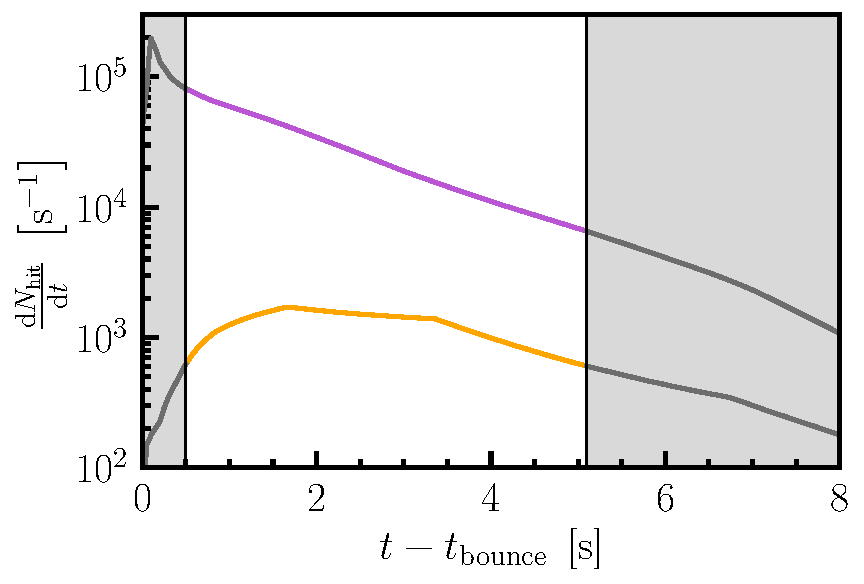
\includegraphics[width=0.47\textwidth]{figures/100MeV_HNL_hits-v-time.pdf}
%     \caption{\textbf{\textit{Hits versus time.}}}
%     \label{fig:hvt_100MeV}
% \end{figure}

% Having appropriately treated the flux at Earth, we can then take the number of hits created by the SM and neutrino fluxes as well as by the SM background, we may now turn to converting the hits to a sensitivity.
% In our study cases, the fluxes---and thus the hits in the detector---have different temporal profiles, see Fig.~\ref{fig:hvt_100MeV}.
% We then consider hits arriving within a certain time window defined by $t_{\mathrm{min.}}$ and $\Delta t$, where these times are measured relative to the so-called bounce time when the first neutrinos from the SN reach the detector.
% In practice, this time can be difficult to reconstruct, and so we consider time bins that are 0.1~s wide, well larger than the uncertainty on the SN start time.
% I NEED TO MAKE SURE THIS IS TRUE...
% We then consider the test given by:
% $$
% -2\log\mathcal{L} = 2\left[N_{\mathrm{exp.}} - N_{\mathrm{obs.}} + N_{\mathrm{obs.}} \log\left(\frac{N_{\mathrm{obs.}}}{N_{\mathrm{exp.}}}\right)\right]
% $$
% where $N_{\mathrm{exp.}}$ is the number of events expected from a given model and $N_{\mathrm{obs.}}$ is the number of neutrinos that would be observed in the SM only case.
% We then say that we are sensitive to a given model then this test statistic exceeds 3.841.
% See Fig.~\ref{fig:sensitivity_heatmap} for an example of the test statistic as a function of these two variables for two different models.

% \begin{figure}
%     \centering
%     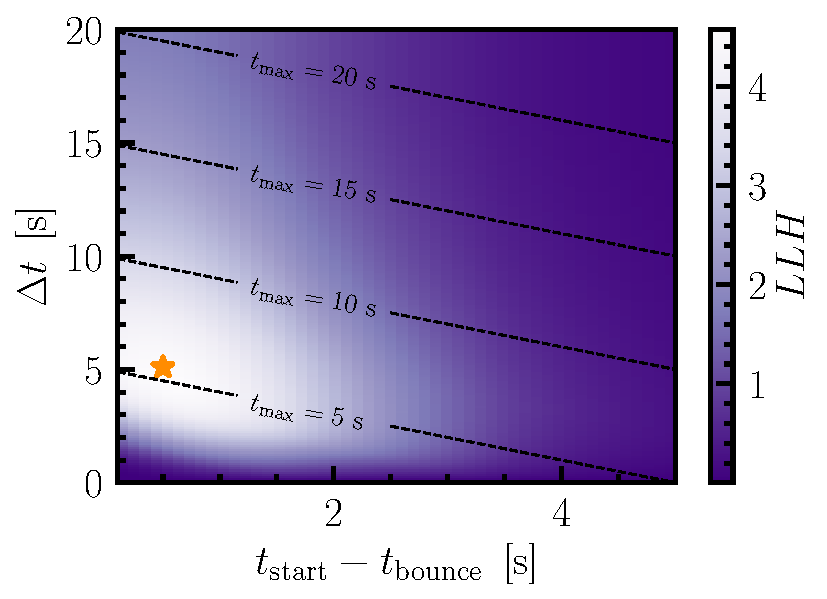
\includegraphics[width=0.47\textwidth]{figures/100MeV_sensitivity_heatmap.pdf}
%     \caption{\textbf{\textit{Test statistic as a function of $t_{\mathrm{start}}$ and $\Delta$t.}
%     }}
%     \label{fig:sensitivity_heatmap}
% \end{figure}
% \textbf{\textit{Statistical Treatment and Sensitivity}}---
% \lipsum[10-12]


\textbf{\textit{Results}}---
\begin{figure}[t!]
    \centering
    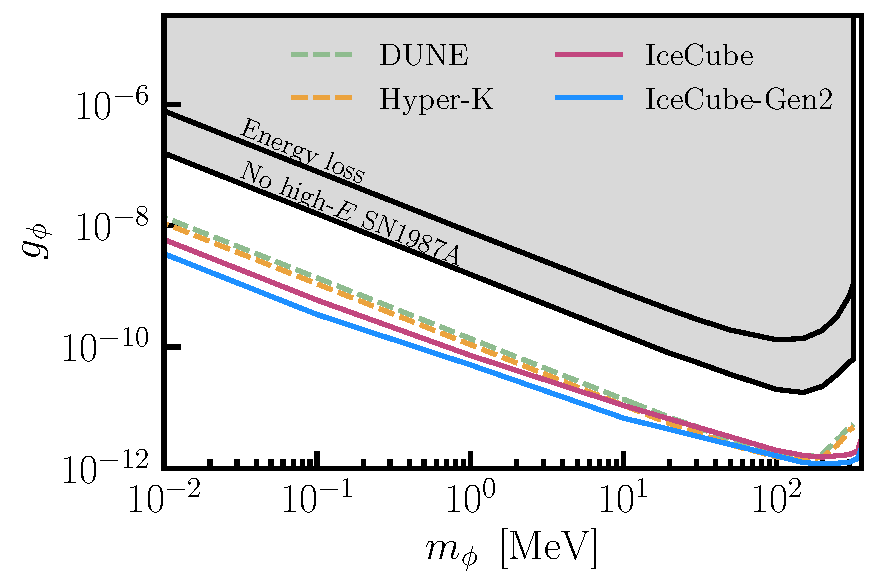
\includegraphics[width=0.47\textwidth]{figures/majoran_sensitivity}
    \caption{\textbf{\textit{Exclusion sensitivities for the Majoron case.}}
    The lines on this plot show the exclusion sensitivity for IceCube, and two next-generation neutrino experiments, Hyper-Kamiokande and DUNE.
    Additionally, we also show the reaches by SN cooling (blue) and by the lack of observation of high-energy neutrinos from SN1987A (grey) \cite{Fiorillo:2022cdq}, with the width of the lines quantifying uncertainties from SN modeling.
    }
    \label{fig:sensitivity}
\end{figure}
Looking for rapid raises within various time windows at neutrino telescope in the occurrence of future nearby SN explosion will provide exceptional tests of the parameter space. Assuming the SN event happens in the galaxy at a distance $D_{\rm SN}=\unit[10]{kpc}$, which is not unlikely~\cite{Reed:2005en,Rozwadowska:2020nab}, we consider the currently operating IceCube neutrino observatory as an example. 
The expected exclusion limit are shown in \cref{fig:sensitivity} (dark red) if no excess of hits on top of those from background noise and the standard neutrino flux were observed. JUNO expected to start taking data soon, while DUNE and Hyper-K requiring longer time to start operating, will be able to test the parameter of Majorons by looking for high energy neutrino following \cite{Fiorillo:2022cdq} if such SN event happens during their operation time. We present the estimated reaches of JUNO, DUNE and Hyper-K in \cref{fig:sensitivity} as xxx, red and orange lines, respectively, leaving aside careful detector analysis, together with current limits \cite{Fiorillo:2022cdq} from the aforementioned energy loss requirement (blue band), and non-observation of high energy neutrinos from SN 1987A (gray band) in \cref{fig:sensitivity}. 

We observe that while for the intermediate mass region, the constraints from IceCube are comparable to that from DUNE and Hyper-K, at both low mass region $m_\phi \lesssim \unit[10]{MeV}$ and high mass region $m_\phi \gtrsim \unit[200]{MeV}$, IceCube can provide stronger constraints. This is the outcome we expect. For light $\phi$ case with negligible time delay, the neutrino signals can  arrive at the detector even before the peak of standard neutrino flux arrives. The resulting hits would appear in a time window separated from that when most of standard flux contribution appears, as we show in the left panel of \cref{fig:hits_and_likelihood}, thus enhancing the reaches. On the high mass end, neutrino signals will arrive much later than the standard case, where a time window at late time can be considered to reduce the standard neutrino contaminations. 

Uncertainties on the analysis from different modeling SN explosion are minor, as studies in \cite{li2023old} and potential discrepancies between data and modeling are unresolved questions. Nevertheless we point out that the discrepancy could be within $2\sigma$ level which will only change our exclusion limit by a small factor.

\textbf{\textit{Outlook}}---
we can also study axion cases, mixing cases with this strategy. Pre-supernova bouncing.

\begin{acknowledgments}
We would like to thank xxx for stimulating discussions about this work. Y.-Y. L is supported by the NSF of China through Grant
No. 12247103 and Grant No. xxx.
\end{acknowledgments}

\bibliography{ic_sn_hnl}

\appendix
\section{Appendix A: Dipole Magnetic Moment Portal}
\begin{figure}[t!]
    \centering
    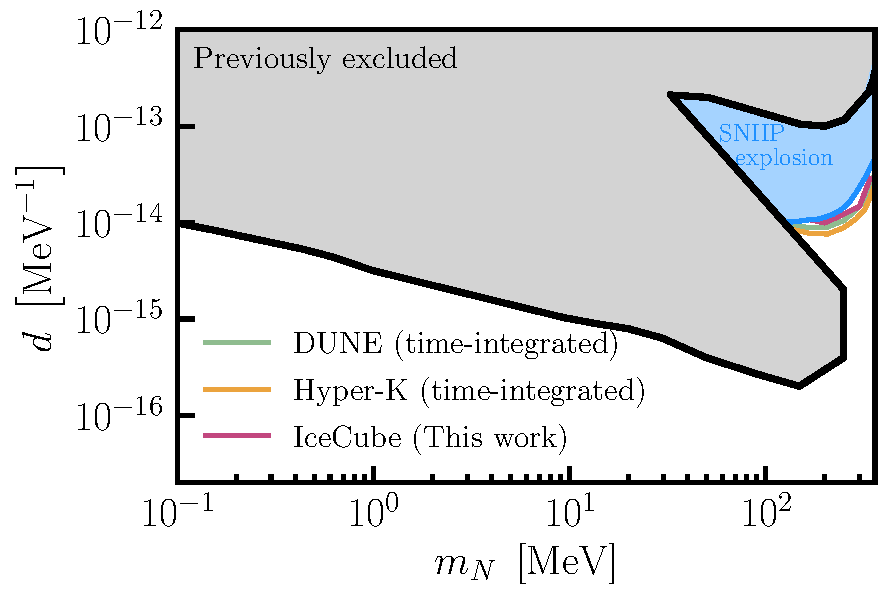
\includegraphics[width=0.47\textwidth]{figures/magnetic_moment_sensitivity}
    \caption{\textbf{\textit{Exclusion sensitivities for the magnetic moment case.}}
    The lines on this plot show the exclusion sensitivity for IceCube, and two next-generation neutrino experiments, Hyper-Kamiokande and DUNE. The shaded regions are excluded by the energy loss constraints, non-observation of photon and neutrino signals from SN1987A studied in \cite{Brdar:2023tmi} and by constraints on the energy release from SN explosion \cite{PhysRevLett.128.221103, Chauhan:2023sci, chauhan2024probing}. \yy{need to update the cyan shaded region as previously excluded using results in \cite{chauhan2024probing}.}
    }
    \label{fig:magnetic_moment_sensitivity}
\end{figure}
The first scenario under consideration is active-to-sterile neutrino transition magnetic moment described by \cite{Magill:2018jla,Brdar:2020quo,Brdar:2023tmi}
\begin{align}
    \mathcal{L} \supset \sum_\alpha d_\alpha \bar{N}\sigma_{\mu\nu} \nu^{\alpha} F^{\mu\nu}-\frac{M_N}{2} \bar{N}^c N + \text{h.c.}\,,
    \label{eq:Lag}
\end{align}
where $\nu^{\alpha}$ and $N$ represent active and sterile neutrinos, respectively. Further, $F^{\mu\nu}$ is the field strength tensor of the electromagnetic field and $d_\alpha$ is the dimensionful coefficient of this dimension-5 term and $M_N$ is sterile neutrino mass. We will abbreviate $d_\alpha \equiv d$ given that we assume flavor universal interaction. We consider the two production channels for $N$ inside the SN: $\nu e^- \to N e^-$ at lower energies and $\nu \gamma \to N$ for larger active neutrino energies. We also point out by neglecting the $N$ production channel $\nu p^+\to N p^+$ inside supernove, the limits we obtained are conservative. Both processes occur due to the interaction term in \cref{eq:Lag}; after $N$ are produced, they decay to active neutrinos and photons which is again realized through the same term in the Lagrangian, with the decay width for $N\to\nu\gamma$ given by $\Gamma_N = 6d^2 M_N^3/4 \pi$ \cite{Plestid:2020vqf}. The limits from IceCube are shown in \cref{fig:magnetic_moment_sensitivity}, together with previously excluded regions by energy loss, non-observations of photons and neutrinos from SN1987A \cite{Brdar:2023tmi}, and constraints on the energy release from SN explosions \cite{PhysRevLett.128.221103,chauhan2024probing}.
We notice that the time delay near the exclusion boundary are typically of $\Delta t \sim \mathcal{O}(1)$ sec, which is longer than the standard $\bar{\nu}_e$ peak luminosity time scale and is not expected to improve over DUNE and Hyper-K performance. 

\end{document}

% Outline
- Introduction: 
- Detector response
  - What kind of noise, Standard neutrino
  - Atm. background reduction ?
- SNEWPY treatment for general models the pipeline etc.
  - The two models that we have condsidered Lagrangians
  - fluxes and results for them
- Conclusion
  - IC is useful for SN
  - Use our software